
%----------------------------------------------------------------------
\section{Experiment Setup}
%----------------------------------------------------------------------

%Our main focus is to evaluate different strategies for preprocessing and query evaluation. For instance, the threshold of “Is hot-structure” part in the diagram,  selection policy for materialized substructures in “Cube-Planner” and “Structure-Planner” , different heuristics when ranking sub-structures during decomposition in “Decomposition and Joining” etc.

There are two purposes of our experiments. First, to compare query processing efficiency of our system with naive Neo4j system. Second, to test how different settings (of parameters and choices of strategies) in our solution affect query processing efficency. Experiments were run on a same set of queries on a same dataset. For datasets, we chose to use real-world datasets. As For queries, we wrote queries with real meanings instead of generating random queries. 

%----------------------------------------------------------------------
\subsection{Datasets}
%----------------------------------------------------------------------

We used a StackOverFlow dataset in our experiment. We created this dataset using raw information from https://archive.org/details/stackexchange. The dataset contains user-contributed content (such as user information, posts etc) on www.stackoverflow.com. The dataset contains 10 different node labels and 12 different edge labels.  Figure \ref{fig:5:1} shows a meta graph of 7 nodes and 8 edges which were involved in our experiments. StackOverFlow dataset is a large dataset which contains over 300 million nodes and more than 400 million edges. Its size on hard disk is 44.5GB. 

\begin{figure}[H]
	\centering
	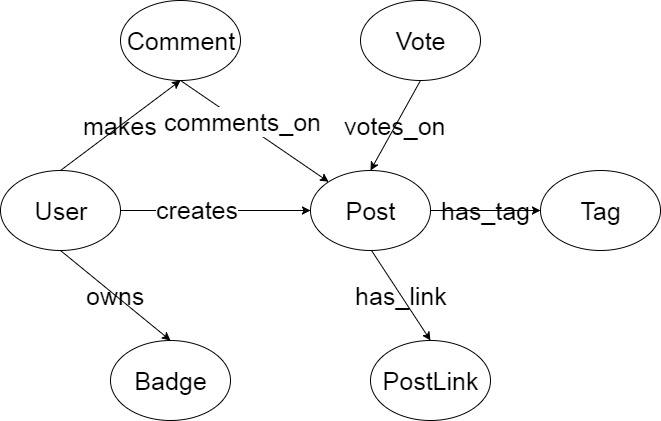
\includegraphics[scale=0.5]{pic/MetaGraphExperiment (1).jpg}
	\caption{A meta graph of StackOverFlow dataset.}
	\label{fig:5:1}
\end{figure}  


%----------------------------------------------------------------------
\subsection{Query Workloads}
%----------------------------------------------------------------------
24 queries of real meanings were written into a query pool. We randomly selected 12 queries as previous workload, leaving the rest 12 ones as future workload. Queries are listed below.


\\\textbf{Previous WorkLoad:}

User-Post: User.UpVotes, Post.Score=10

User-Post: User.UpVotes, (AVG)Post.Score

User-Post: User.Age, (SUM)Post.ActiveMonth

User-Post: User.CreationDate_Year, Post.PostTypeId=1

Badge-User, User-Post, Post-Tag: Tag.TagName, User.CreationDate_Year=2017

Badge-User, User-Post, Post-Tag: Tag.TagName, Badge.Name

Badge-User, User-Post:Badge.Date_Year,(AVG)Post.Score

Badge-User, User-Post:Badge.Class,(AVG)Post.ActiveMonth

User-Post, Post-Tag: (AVG)User.Age, Tag.TagName

User-Post, Post-Tag: (AVG)User.UpVotes, Tag.TagName=Java

User-Post, Post-Vote: (AVG)User.UpVotes, Vote.VoteTypeId

Post-Comment, Post-PostHistory: PostHistory.PostHistoryTypeId=5, (AVG)Comment.Score


\\\textbf{Future WorkLoad:}

User-Post: User.CreationDate_Year=2017, Post.PostTypeId

User-Post: (AVG)User.UpVotes,Post.Score

User-Post: Post.ActiveMonth, (AVG)User.Age

User-Post: User.CreationDate_Year

Badge-User, User-Post, Post-Tag: Tag.TagName, Badge.Class

Badge-User, User-Post, Post-Tag: Tag.TagName, Badge.Date_Year

Badge-User, User-Post:Badge.Name, Post.PostTypeId

User-Post, Post-Tag: User.UpVotes, Tag.TagName, Post.PostTypeId=2

User-Post, Post-Tag:User.CreationDate_Year, Tag.TagName

Post-PostLink, Post-Tag: Tag.TagName=database, PostLink.LinkTypeId

Badge-User, User-Comment: Badge.Class, (AVG)Comment.Score

Post-Tag, Post-Vote: Tag.TagName




%----------------------------------------------------------------------
\subsection{System Setting}
%----------------------------------------------------------------------

We ran all the experiments on a Linux cluster machine with main memory of 256GB. Our system is implemented in Java. We set initial Java vitual machine memory as 100GB and maximum Java vitual machine memory as 200GB.

%----------------------------------------------------------------------
\subsection{Neo4j Configuration}
%----------------------------------------------------------------------
We used Neo4j Community v3.1.3 as database server. Neo4j's initial memeroy size is set as 60GB and maximum memeroy size as 200GB. We used Neo4j's official Java driver to interact with Neo4j server.

%----------------------------------------------------------------------
\section{Aspects of Interest}
\label{Aspects of Interest}
%----------------------------------------------------------------------

As we mentioned, there are two purposes of our experiments. The second purpose requires tests on how different settings in our system affect query processing efficency. We list the following aspects of interest which were tested. Default setting for each aspect is also presented. For variable control purpose, in each test all aspects were set to default settings, except for the only one aspect on which we would test.  

\textbf{Materialization}
\begin{itemize}

\item  Memory limit, i.e. $\sigma$ in Algorithem \ref{alg:StructurePlanner}. Default setting: 6GB.

\item  Algorithm in materialized view selection \ref{Materialization Part}. For cuboid selection, we  campared CubePlanner \ref{sec:CubePlanner} with ``Patial Materialization'' algorithm (PMA) proposed in Graph Cube \cite{DBLP:conf/sigmod/ZhaoLXH11}. For substructure selection we will compared StructurePlanner \ref{Structure Planner} with frequent pattern mining algorithm (FPM). Default setting: CubePlanner and StructurePlanner.

\item Frequency threshold for identification of “hot structures”, i.e. $\omega$ in Algorithm \ref{alg:1}. Default setting: 4. Section \ref{Frequency Threshold} explains why setting $\omega$ as 4. 

\item Storage for merialized views. We will compare main memory storage v.s. hard disk storage. Default setting: main memory storage.

\end{itemize}

\textbf{Future Query Processing}
\begin{itemize}
\item  Choice of score functions in ranking substructures during ``Substructure Selection'' \ref{Substructure Selection}, i.e. $h(s)$ in Algorithm \ref{alg:SelectSubstrucre}. Default setting: $h(s)$ returns the score of $s$ calculated in StructurePlanner (as result of line 11 in Algorithm \ref{alg:StructurePlanner}). 

\item  Choice among using $Decompose\_Join$, $Decompose\_Join^{*}$ and $Decompose\_Join^{+}$ in ``Decomposition and Join'' \ref{Query Decomposition}. Default setting: $Decompose\_Join$.

\end{itemize}

Besides, we also ran experiments on the smaller dataset to see how performance varies in datasets of different sizes.  

%----------------------------------------------------------------------
\section{Results and Discussion}
\label{Results and Discussion}
%----------------------------------------------------------------------
In this section, results of experiments are presented and explainations of results are given. 

%----------------------------------------------------------------------
\subsection{Our System vs. Neo4j Baseline}
%----------------------------------------------------------------------
We used default settings for our system and compared  with naive Neo4j system over processing time for the future workload (12 queries).


\begin{figure}[H]
	\centering
	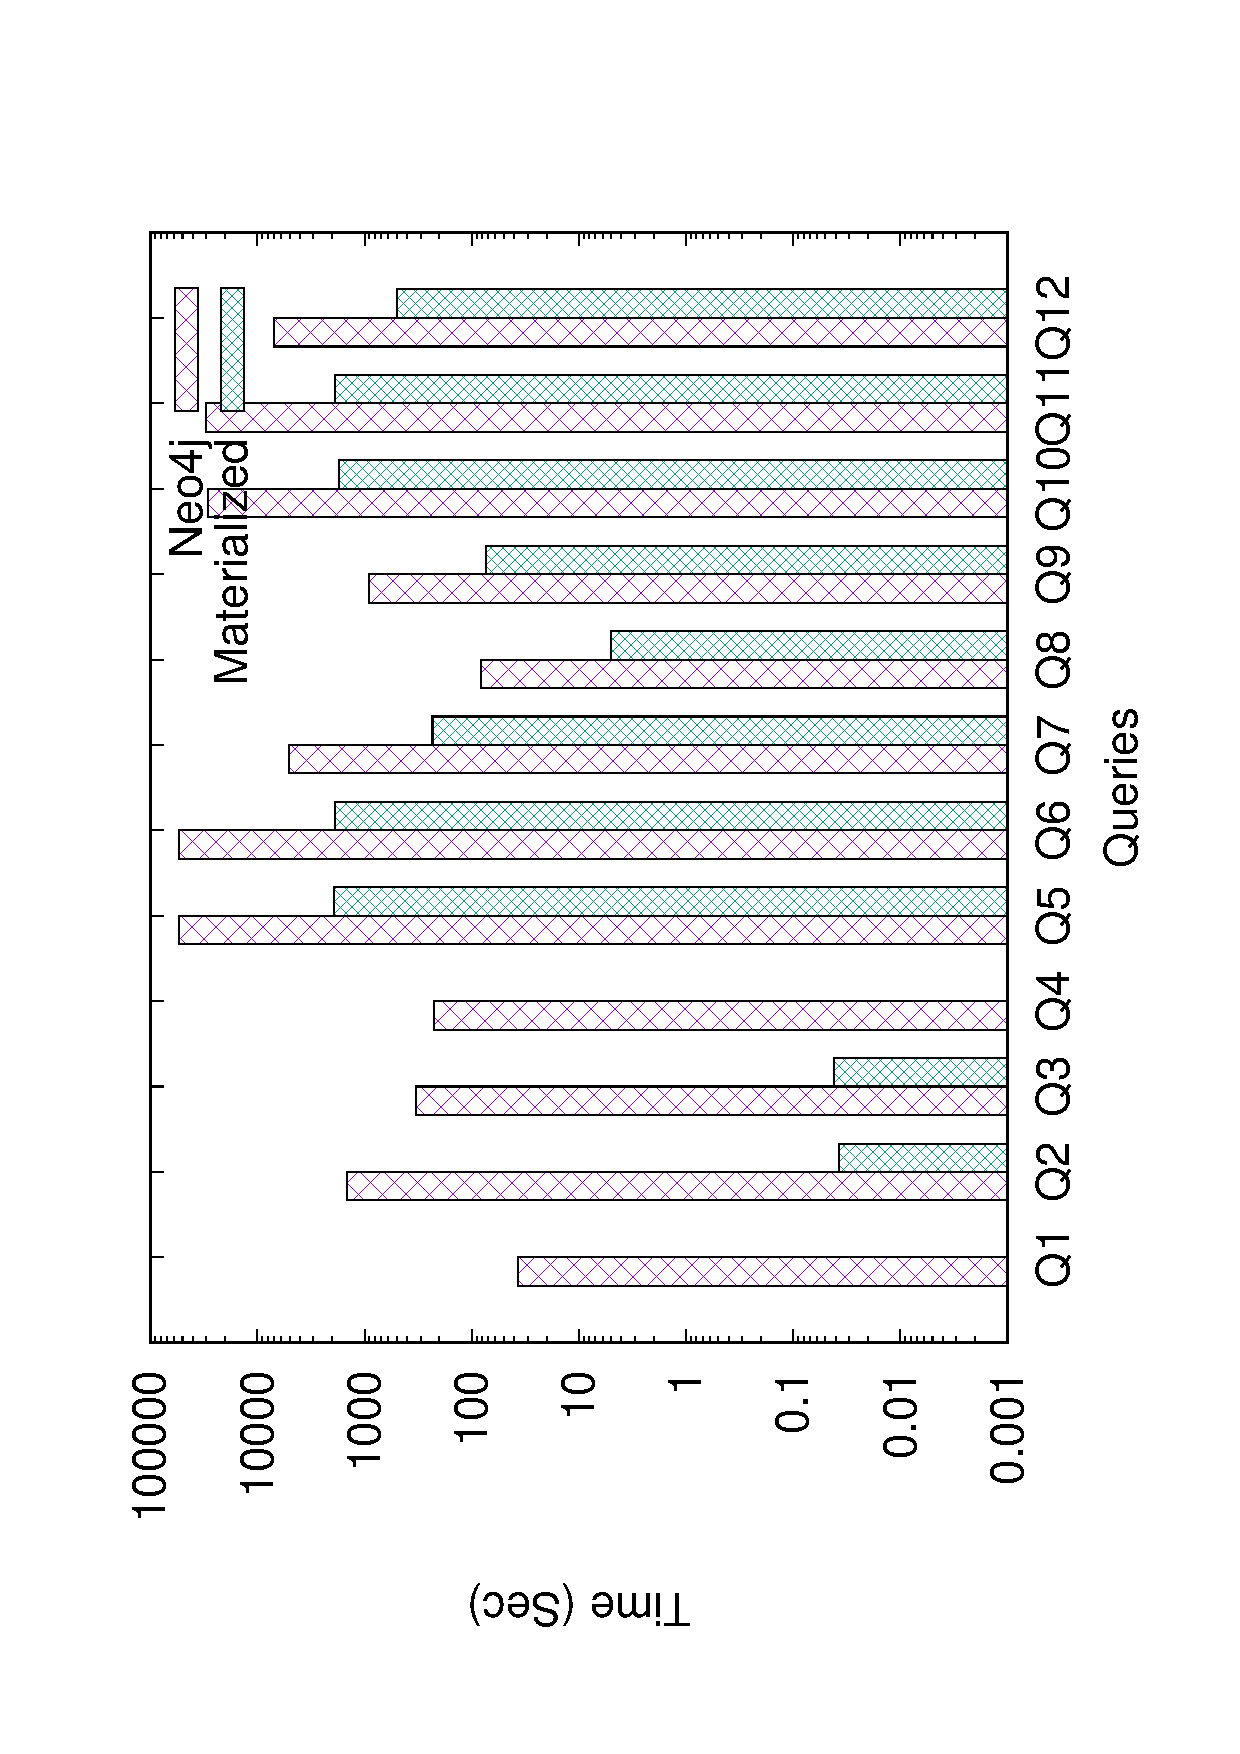
\includegraphics[scale=0.5, angle=270]{plot/neo4j}
	\caption{Processing time for future workload by our proposed solution v.s. Neo4j.}
	\label{fig:neo4j}
\end{figure}

Figure \ref{fig:neo4j} shows processing time for 12 future queries by both our system and Neo4j. We see that with a cost of 5.7GB materializd view storage, which is acceptable considering size of the dataset, our solution achieved remarkable efficiency improvement.

\begin{figure}[H]
	\centering
	\includegraphics[scale=0.5]{"pic/MetaGraphExperiment_Hot (1)"}
	\caption{Substructure selected by StructurePlanner.}
	\label{fig:metagraphexperimenthot}
\end{figure}

We detail how our system worked. First, \textit{User-Post} was identified as ``hot structure''. As a result, P1 - P4 were passed to CubePlanner and P5 - P12 were passed to StructurePlanner. Cuboids selected by CubePlanner are \textit{User-Post: User.Age, Post.ActiveMonth}; \textit{User-Post: User.CreationDate\_Year, Post.PostTypeId}; \textit{User-Post: User.UpVotes, Post.Score}. Figure \ref{fig:metagraphexperimenthot} highlights substructures S that StructurePlanner selected:  \textit{User-Post} (s1), \textit{Post-Tag} (s2) and \textit{Badge-User} (s3). From observation of previous workload, we can tell that StructurePlanner made a wise decision as these three substructures are able to cover most of previous queries. 

We give explainations on performance differences by each query. Avarage improvement rate for Q1 - Q4 is around 7000. This is because Q1 - Q4 got hit by C (``cuboid hit''). As a result processing time is reduced to a much greater extent than Q5 - Q12 (which did not get ``cuboid hit''). Note that time complexities of cuiboid aggregation and substructure joins are in different scales. Time complexity of cuiboid aggregation is bounded by production of cardinalities of involved properties. When it comes to substructure joins, however, time complexity is related to the actual data sizes. Q5 - Q9 are totally covered by S. As a result no ``complementary components'' were fetched from database.  Q10 - Q12 are partially coverd by S.  ``Complementary components'' were fetched from database, which increased time cost. As a result improvement rate for Q5 - Q9 ranges from around 10 to more than 30, while improvement rate for Q10 - Q12 ranges around 10, which is lower. To conclude, our system greatly improved query processing efficency. Improvement rates vary in different senerios of cuboid and structure ``hits''.




%----------------------------------------------------------------------
\subsection{Frequency Threshold}
\label{Frequency Threshold}
%----------------------------------------------------------------------
Frequency threshold $\omega$ has an important effect on query processing efficiency. A change of $\omega$ may result in changes of ``hot structures'', followed by changes in inputs for CubePlanner and StructurePlanner. This will further result in different materialized view selection and finally different query processing performance. As indicated in Section \ref{Overview of Materialization Part}, $\omega$ serves as a minimum bar to convince that building a cuiboid over a ``hot structures'' is worthy (``cuboid hit'' assured). We think 4 is an appropritate choice for $\omega$ in our test case considering frequency count of structures in previous workload (as shown in the below table). 

\begin{center}
	\begin{tabular}{ | c | c |}  
		\hline
		Structure	&Frequency	\\ \hline 
		\textbf{User-Post} 	&\textbf{4} \\ \hline
		Badge-User, User-Post, Post-Tag 	&2 \\ \hline
		Badge-User, User-Post	&2 \\ \hline
		User-Post, Post-Vote	&2 \\ \hline
		Badge-User, User-Comment	&1 \\ \hline
		Post-Comment, Post-Vote	&1 \\ \hline
	\end{tabular}
	\end {center}

Suppose we lower $\omega$ to 2. \textit{Badge-User, User-Post, Post-Tag} will be ``hot structure''. As a result, cuboid selection over \textit{Badge-User, User-Post, Post-Tag} will be considered based on merely two queries (P5 and P6). Notice that Q5 and Q6, which have structure \textit{Badge-User, User-Post, Post-Tag}, will never get ``cuboid hit''. This is because properties Badge-Class in Q5 and Badge-Date_Year in Q6 did not even appear in P5 and P6. That is to say, in this case any cuboid selected over \textit{Badge-User, User-Post, Post-Tag} will be useless. In addtion, when $\omega$ is set to 2, input for StructurePlanner will be only two queries (Q11 and Q12). Note that structure frequency counts of these two queries are both 1. In other word, these are the most ``random'' queries. Note that the idea of StructurePlanner is discovery of useful substructures based on a sufficent number of ``less hot'' queries. In this case two ``random'' queries is not an ideal input for StructurePlanner.  

On the other side, suppose we increase $\omega$ to 5, then there will be no cuboid materialized. As a result Q1 - Q4 will be processed using substructure materialization (s1). Despite this is still faster than naive Neo4j system, the outstanding improvement rate of ``cuboid hit'' cannot be achieved. 

Figure \ref{fig:omega} presents total processing time under different settings of $\omega$. We reach our conclustion that $\omega$ did have a significant effect over system performance. Actually determination on the value of $\omega$ is an interesting classification problem (based on frequency count). However we will leave this topic to future work since it is not the main focus of our work. 

\begin{figure}[H]
	\centering
	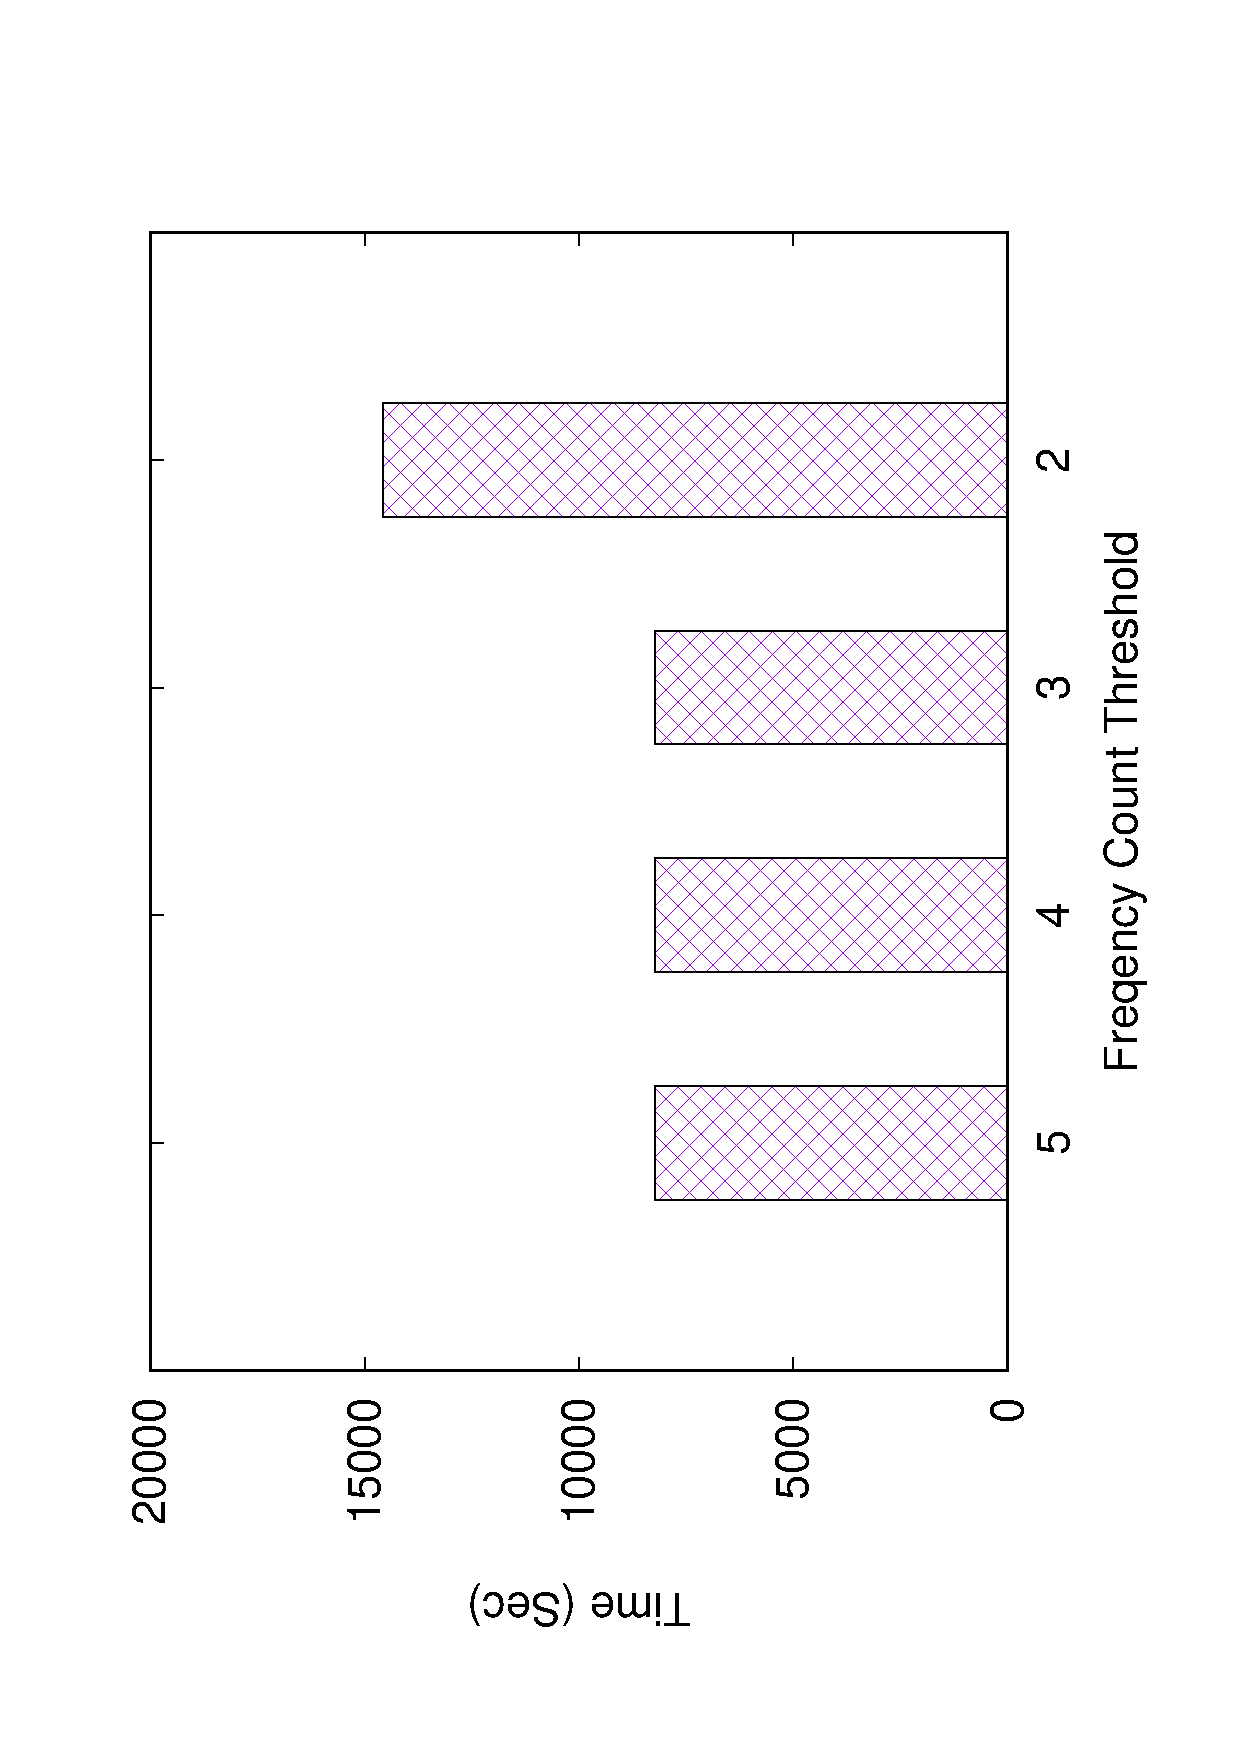
\includegraphics[scale=0.5, angle=270]{plot/omega}
	\caption{Total processing time under different settings of $\omega$.}
	\label{fig:omega}
\end{figure}


%----------------------------------------------------------------------
\subsection{Space Cost Limit}
%----------------------------------------------------------------------
Our default setting \ref{Aspects of Interest} sets space cost limit for materialized views $\sigma$ to be 6GB and the actual space cost of materialized views is 5.7GB. If we change $\sigma$ we may get different materialized views thereby different efficiency performance. Figure \ref{fig:limit} shows how total processing time varied by different actual space costs (which were caused by setting $\sigma$ to 6GB, 4GB and 2.5GB). From the figure we see that with more views being materialized, total processing time is reduced. However the maginal effect from new views decreased as more views were materialized. This indicates that our Greedy Selection Framework successfully picked candidates by their maginal benefits.

\begin{figure}[H]
	\centering
	\includegraphics[scale=0.5, angle=270]{plot/limit.eps}
	\caption{Efficiency v.s. Space Cost}
	\label{fig:limit}
\end{figure}

%----------------------------------------------------------------------
\subsection{Storage for Merialized Views}
%----------------------------------------------------------------------
In the default setting \ref{Aspects of Interest}, materialized views are stored as objects in main memory. This provides fast access to the views but causes a main memory storage cost. Alternatively materialized views can be serialized and stored as files on hard disks. Figure \ref{fig:disk} shows that hard disk storage did not perform as fast as main memory storage, but the drop in efficency is acceptable. Such drop in efficency is owing to I/0 overhead in reading materialized views from files.

 One interesting question is since eventually materialized views are be read into main memory, what is the point of storing them in files? Our answer is that in cases when main memory is far too small for holding all selected views, hard disk materialization provides a lower level of storage of sufficent volume.
 
\begin{figure}[H]
	\centering
	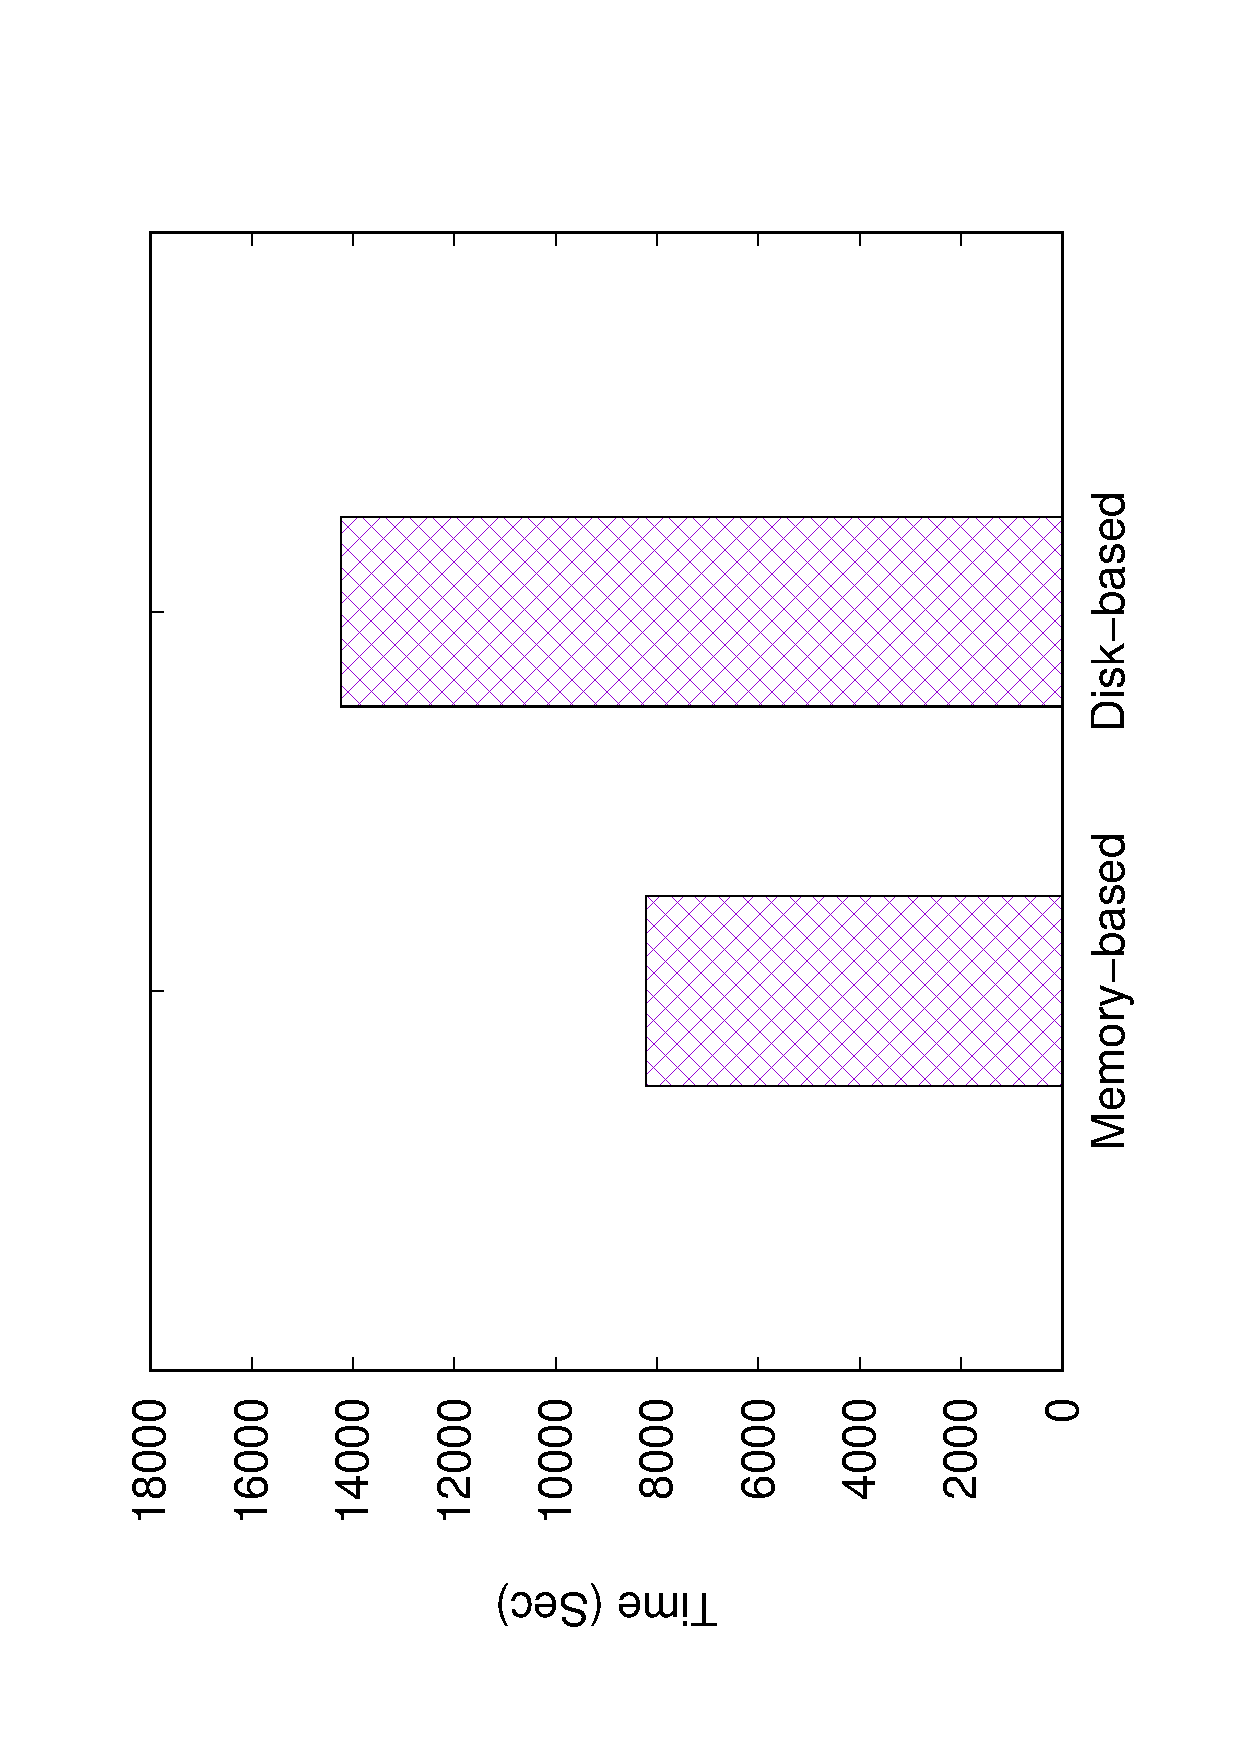
\includegraphics[scale=0.5, angle=270]{plot/disk}
	\caption{Main memory storage v.s. hard disk storage}
	\label{fig:disk}
\end{figure}

%----------------------------------------------------------------------
\subsection{CubePlanner v.s. PMA}
%----------------------------------------------------------------------
We compared CubePlanner \ref{CubePlanner} in our solution with PMA in Graph Cube \cite{DBLP:conf/sigmod/ZhaoLXH11}. Figure \ref{} and \ref{} show that CubePlanner outperformed PMA in both query processing efficency and space cost. 

Acutally both two approaches are considered as implementations of Greedy Selection Framework \ref{s:Greedy Selection Framework}. We reveal differences between the two implementations. CubePlanner uses the ratio of marginal benefit over space cost as a score for candidate ranking (line 11 inAlgorithm \ref{alg:SingleCubePlanner}). While PMA only considers maginal benefit. That is to say, space cost does not count in PMA. This gives rise to why CubePlanner outperformed PMA in terms of space cost. Moreover, PMA treats each combination of properties with equal weight, regardless of how many times a combination appeared in previous queries. For example in our test case, combination of {User.UpVotes, Post.Score} appeared twice in previous workload. But PMA would treat {User.UpVotes, Post.Score} with the same weight as those combinations that were not even queried in previous workload (\{User.UpVotes, Post.PostTypeId\} etc). As a result, CubePlanner adopted more information from previous workload and thus made better selection. 

%----------------------------------------------------------------------
\subsection{StructurePlanner v.s. FPM}
%----------------------------------------------------------------------
We compare our algorithm \ref{alg:StructurePlanner} in StructurePlanner with FPM. In FPM we set minimum support to 2 considering frequency count as listed in the table in Section \ref{Frequency Threshold}. These two ways provided different substrcutre selections which led to different processing performance. Figure \ref{fig:fpm} and \ref{fig:fpmspace} show that our StructurePlanner outperformed FPM in both efficency performance and space cost.

\begin{figure}[H]
	\centering
	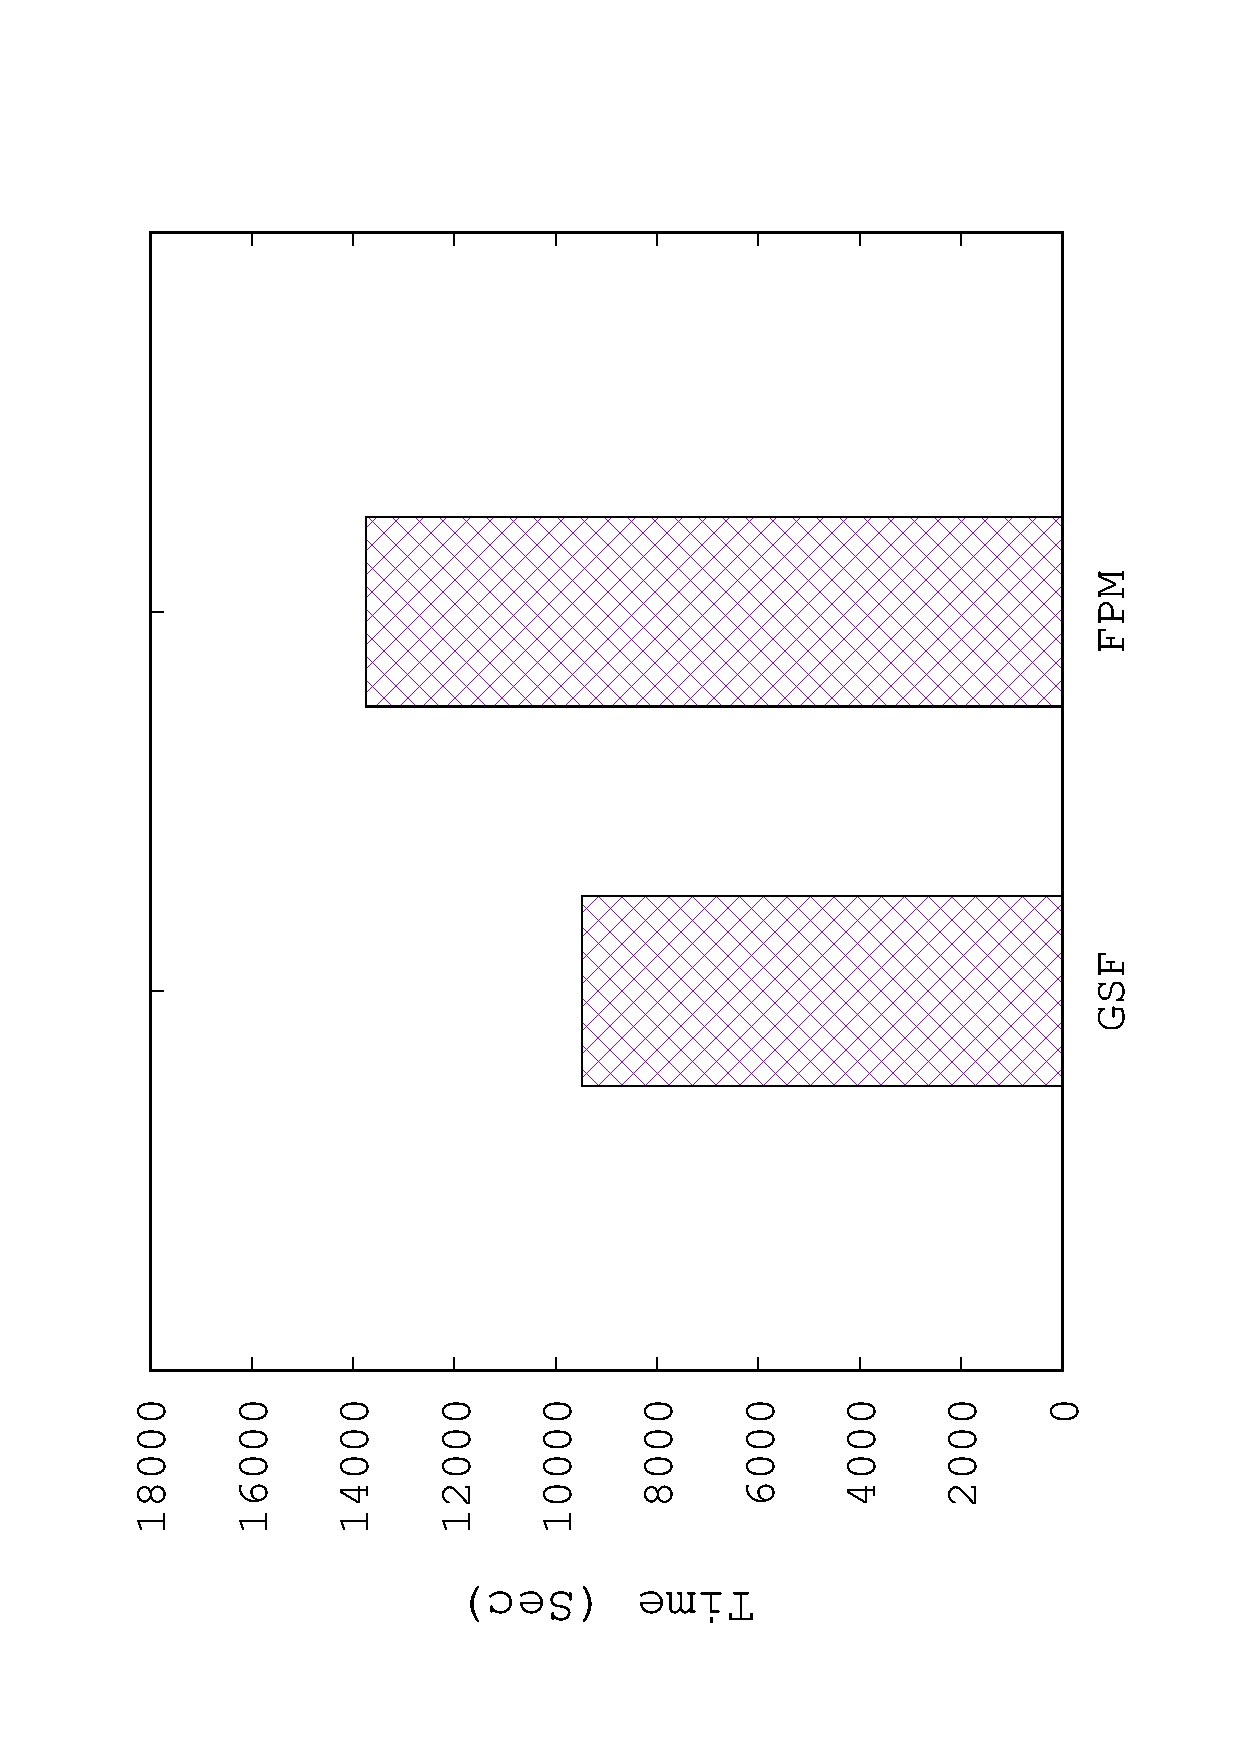
\includegraphics[scale=0.5, angle=270]{plot/fpm}
	\caption{Total processing time: StructurePlanner v.s. FPM}
	\label{fig:fpm}
\end{figure}

\begin{figure}[H]
	\centering
	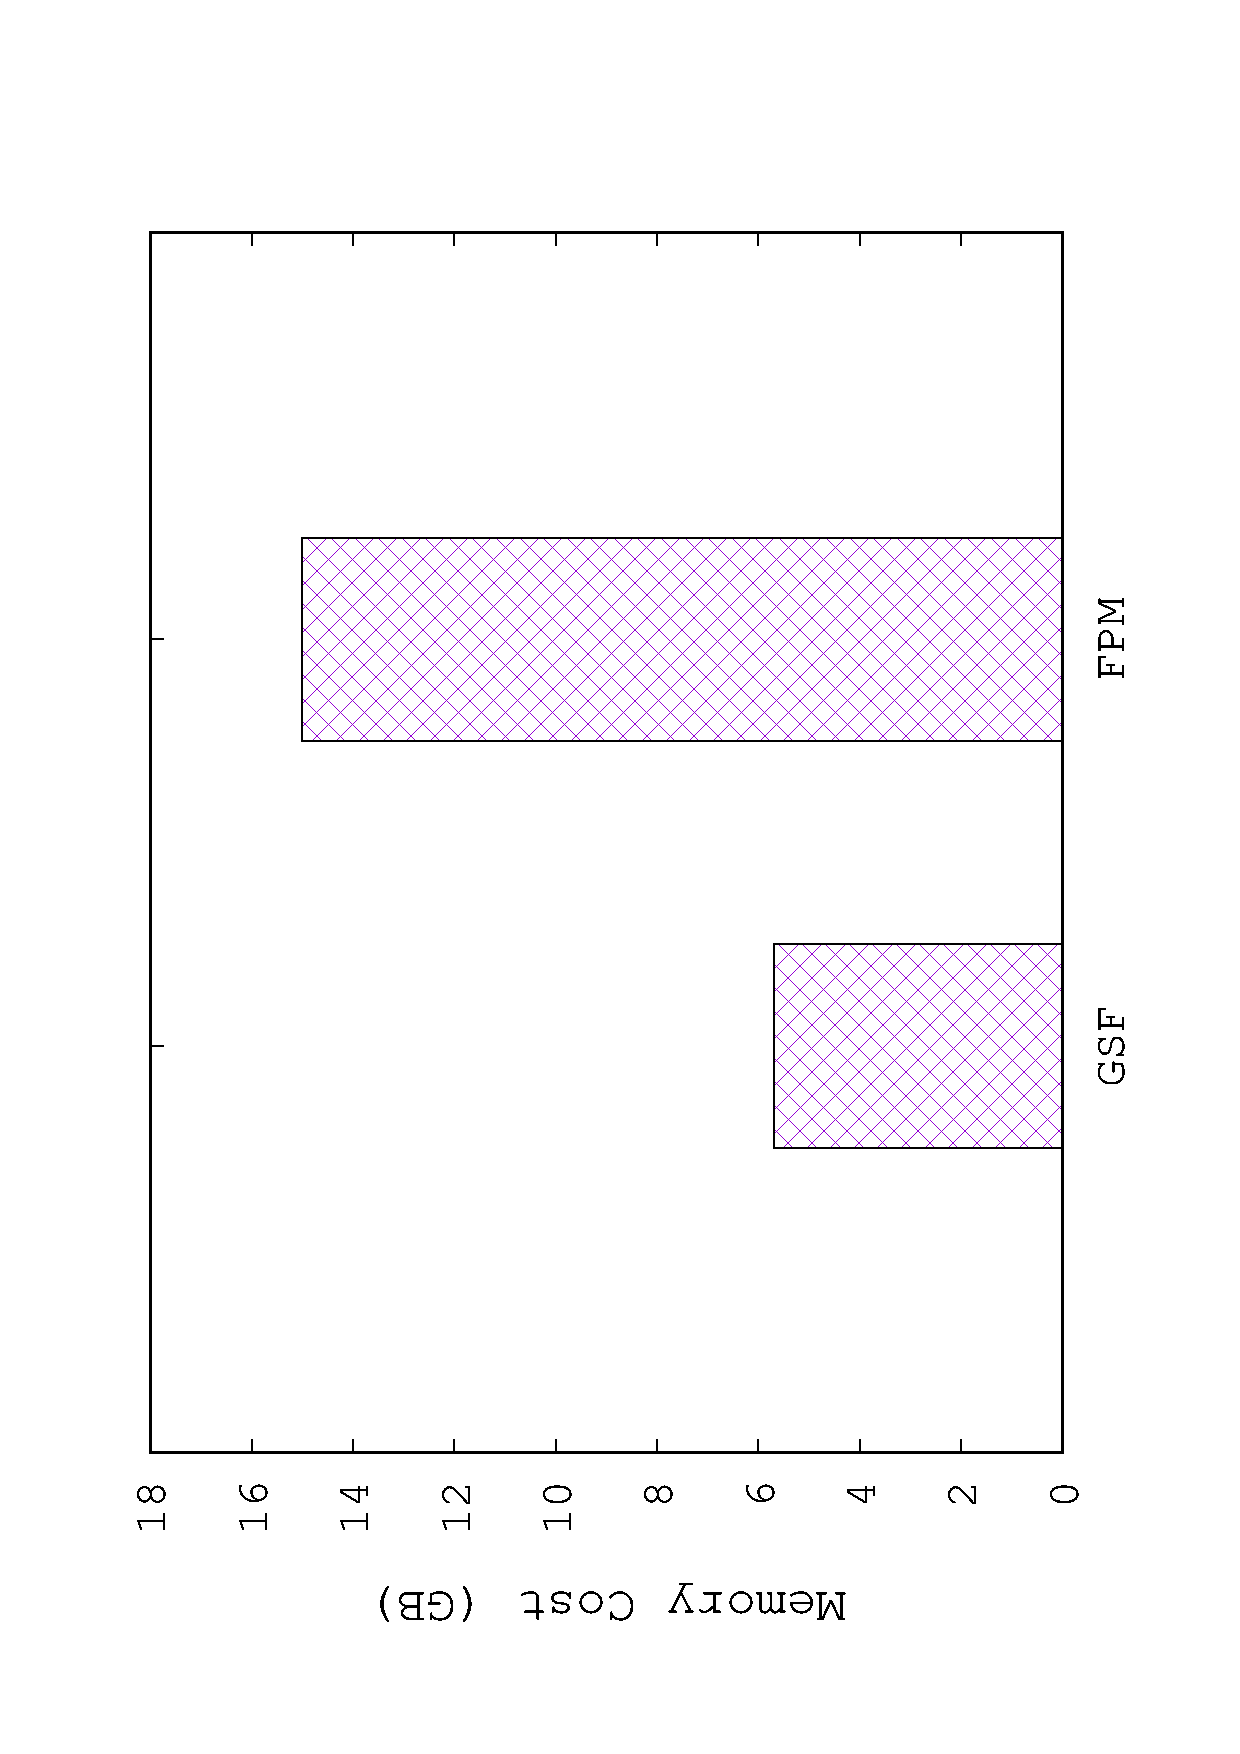
\includegraphics[scale=0.5, angle=270]{plot/fpm_space}
	\caption{Space cost: StructurePlanner v.s. FPM}
	\label{fig:fpmspace}
\end{figure}

Figure \ref{fig:metagraphexperimenthot} highlights three selected substructures by StructurePlanner. As mentioned it is a wise selection as these three substructures were able to cover the most of previous queries. However, Frequent Pattern Mining selected \textit{Badge-User, User-Post, Post-Tag}. This is a bad selection because it was useful only for Q5 and Q6. In addition, materialization of \textit{Badge-User, User-Post, Post-Tag} results in even more space cost than materialization of the three edges seperately (as selected by StructurePlanner). Figure \ref{fig:qfpm} details processing time for each query. FPM only outperformed StructurePlanner on Q5 and Q6. This is because by FPM Q5 and Q6 were processed by direct aggreagation over structure materialization of \textit{Badge-User, User-Post, Post-Tag}, while by StructurePlanner table joins of s1, s2 and s3 was required, which costed more time. However for Q7 - Q12, StructurePlanner outperformed as it got at least patial ``substructure cover'' while selected result of FPM helped nothing.

\begin{figure}[H]
	\centering
	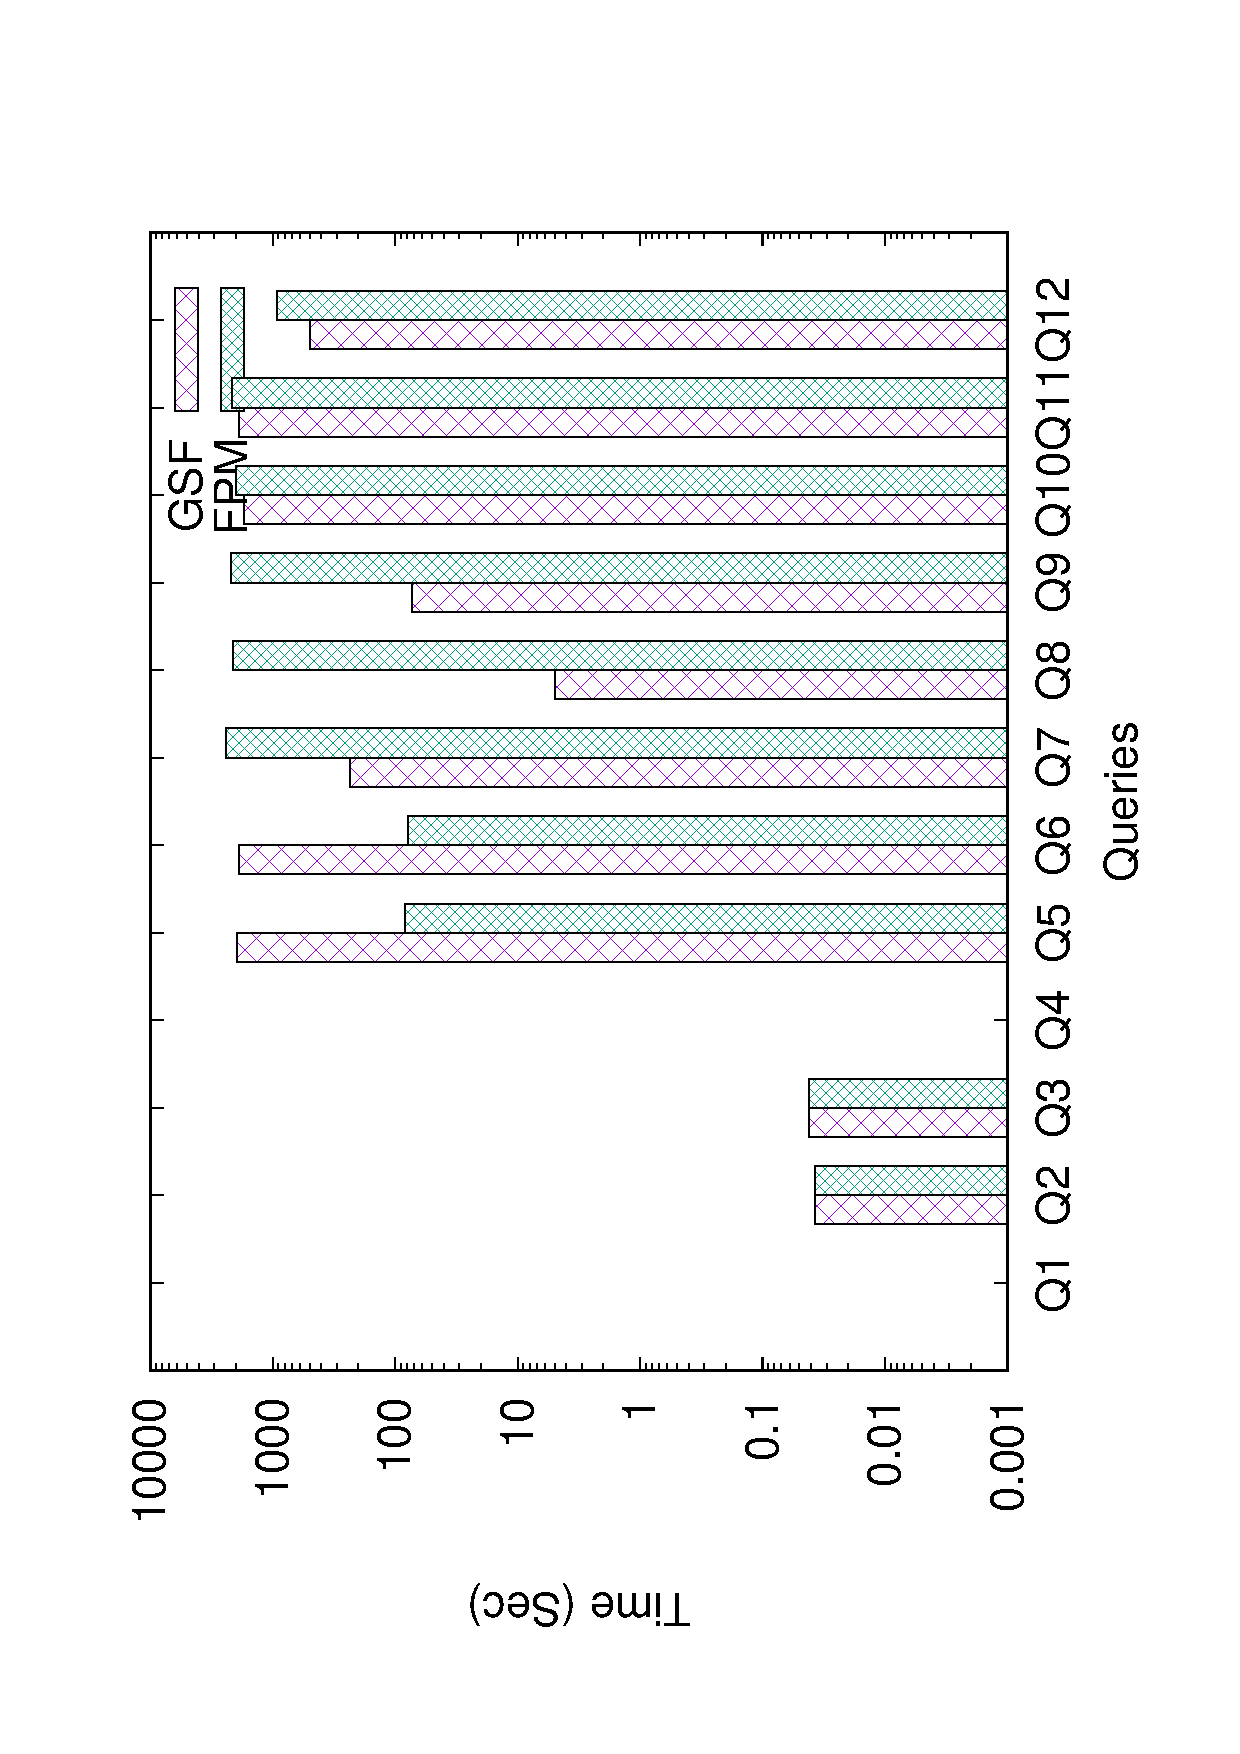
\includegraphics[scale=0.5, angle=270]{plot/qfpm}
	\caption{Processing time for each query: StructurePlanner v.s. FPM}
	\label{fig:qfpm}
\end{figure}


%----------------------------------------------------------------------
\subsection{Substructure Selection}
%----------------------------------------------------------------------

In our experiment, $h(s)$ in Algorithm \ref{alg:SelectSubstrucre} did not make any difference during ``Substructure Selection'' \ref{Substructure Selection}. This is because the three selected substructures do not share any common edge. Note that senerios in Section \ref{Substructure Selection} where multiple valid combinations of materialized substructures exist only happen when materialized substructures have overlaps. 

%----------------------------------------------------------------------
\subsection{Decompose\_Join}
%----------------------------------------------------------------------
We conducted tests on $Decompose\_Join$, $Decompose\_Join^{*}$ and $Decompose\_Join^{+}$ in ``Decomposition and Join'' \ref{Query Decomposition}. Such three different implementations in ``Decomposition and Join'' made a difference in processing Q10 - Q12, as they were patially covered by S and fetching ``complementary components'' from Neo4j was needed. Figure \ref{} provides processing time for Q10 - Q12 by the three approaches. $Decompose\_Join^{*}$ performed much better than $Decompose\_Join$ in Q10. This is because $Decompose\_Join^{*}$ passed candidate IDs of posts with ``database'' tag to Neo4j, which provided a tramendous ``filtering effect'' when fetching \textit{Post-PostLink}. As a result, $Decompose\_Join^{*}$'s time for fetching \textit{Post-PostLink} was greatly reduced. Besides, its time for joining \textit{Post-Tag} and \textit{Post-PostLink} also decreased because table sizes of \textit{Post-Tag} and \textit{Post-PostLink} are smaller than those in $Decompose\_Join$ thanks to the ``filtering effect''. This is reflected in Figure \ref{}, from which joining time is seen to have been saved in $Decompose\_Join^{*}$. However $Decompose\_Join^{*}$ performed badly in Q12. This is because ``filtering effect'' of \textit{Post-Tag} in fetching \textit{Post-Vote} is little. In addition, $Decompose\_Join^{*}$ had a considerable overhead of scanning the table of \textit{Post-Tag} in order to get the set of candidate IDs. This explains why $Decompose\_Join^{*}$ took longer time in processing Q12. Figure \ref{} gives total processing time for Q10 - Q12 by the three approaches. We see that $Decompose\_Join^{+}$ had best overall performance. This is because $Decompose\_Join^{+}$ was able to choose the faster approach when fetching ``complementary components'' from Neo4j in senerios like Q10 and Q12 with only a small cost of ``trial query'' \ref{Query Decomposition}. This is reflected in Figure \ref{}. Note that time cost for ``trial query'' is bounded by a constant sampling size (which was set to 100 in our experiments). It is not proportional to actual data size in the dataset. Figure \ref{} shows that time cost ``trial query''is acceptably small. 

To conclude, ``filtering effect'' is an important facter in performance of these three implementations of ``Decomposition and Join''. In general, $Decompose\_Join^{+}$ is the recommended approach as it is able to make the better of the other two approaches with a small cost of ``trial query''.


%----------------------------------------------------------------------
\subsection{Large DataSet v.s. Small DataSet}
%----------------------------------------------------------------------
Besides StackOverFlow dataset (45.8GB), we also tested on a smaller ``StackExchange-Math'' dataset of size 2.57GB. Like StackOverFlow dataset, StackExchange-Math dataset is about a mathematics Q\&A forum (https://math.stackexchange.com).  The raw data of StackExchange-Math dataset also comes from https://archive.org/details/stackexchange and it has exactly the same schema as StackOverFlow dataset. 

Figure \ref{} compares efficiency improvement rate for large dataset and smaller dataset. We see that our system achieved even better performance on larger dataset. 


